\chapter{Multilab control software}\label{sec:ml_software}
In the years before moving the DTU Space multilab to DTU campus, it became apparent that a completely new software solution was needed for the coating facility. The software controls all stepper motors (cathode shutters and sample ring), gas flow controllers,  cathode power supplies as well as pressure gauge communication.

The original software was made in Visual Basic 6, which Microsoft stopped supporting in 2008. Features that were not build into the software from the start was bolted on at a later stage, resulting in some files with thousands of lines of uncommented code. VB6 also has the drawback that it is single threaded so only one command can be executed at a time, which means that none of the instruments could be read for the log file if e.g. the sample ring was moving. So checking whether there was a plasma dropout on a cathode was not possible while coating a layer, something that can take 30+ minutes.

Everything in the original software solution was controlled in a graphical user interface which made it easy to use, but would only allow for preprogrammed coating types to be made. When it came to make coating investigations for the Athena mission, the linearly graded coatings with top and bilayer required being in front of the computer during the process. For every layer, it was necessary to manually type in a new sample ring speed and start the movement. The coatings took on average 2-3 hours, so it became clear that a new solution was necessary.

\section{Considerations on the new software solution}
Considering the observations from above, a list of requirements for new software was made:

\begin{description}
  \item[Software should run on Linux] To remote control the coating facility in the old software solution, it was necessary to run a remote desktop to control the graphical user interface. The remote desktop requires a relatively large amount of internet bandwidth, something that is not always available. The new software should be controllable over a remote SSH connection using a Bash shell or similar.
  \item[Software should log continuously] Output from cathode power supplies, pressure gauges and flow meters should be read every 5 seconds during a coating. Between coatings, the pressure gauges should be read every 5 seconds and written to a web server. That allows for checking chamber status on a smart phone or computer connected to the internet.
  \item[A coating run should be described in a script] Instead of predefined coating types, the scripts make it possible to produce completely custom multilayer coatings.
  \item[Software should preferably be open source] Open source software is often well documented and flexible. An open source programming language with plenty of extra packages could be Python.
\end{description}

The first attempts at creating new software was directed at Python, since that is just about the most well-documented programming language on the internet, and also where I have the most experience.

It became clear after a while that the real problem was satisfying the second requirement in the list above. All instruments controlled by computer in the multilab are communicated with using serial connections, which will block a line until a command is received by an instrument and a response is returned. In some instruments the response time is up to a second and for the stepper motors, a response is not returned until movement is complete. That is the reason why the old software was unable to read any outputs during the movement of the sample ring.

Python is a single threaded scripting language, so all commands are executed sequentially. There are however software packages for Python that can spawn subprocesses from a queue and read the output of those into another queue. A specific package for multithreading serial communication is Twisted for Python, but after moderately successful attempts it was clear that the solution would be too difficult. The software should be flexible and making a multithreaded python solution with queue systems was both too much work and a bit like reinventing the wheel.

The choice in the end fell on SPEC (by Certified Scientific Software), a software package for X-ray diffraction setups. SPEC is not open source, but requires a license. SPEC is widely used in synchrotron beamlines across the world, and also in the X-ray lab at DTU Space. It is an extremely flexible piece of software, specifically designed to talk to a wide range of instruments at X-ray beamlines. Many types of hardware can be controlled directly from SPEC without the need for drivers, since a direct hardware level communication protocol is build into the software. Commands are typed in on a command line, but can also written into text files (scripts) and the commands can then be executed sequentially by SPEC.

\section{Software architecture of new Multilab control program}
SPEC is, like Python, single threaded. There are however build-in procedures for communicating through the serial protocol and a range of other protocols. SPEC also has the ability to run as a server so commands can be issued to the software using sockets on the system level. By running three separate instances of SPEC at the same time, it became possible to constantly communicate with instruments, write to a logfile, and control the chamber from a main program. The software is set up like the following:

\begin{description}
  \item[SPEC (main program)] The main program, where user-level commands can be typed in. Coating macros are executed from this program. The program has direct control with stepper motors using text-based serial communication\footnote{To use SPEC most efficiently, a direct hardware-level communication should be initiated between SPEC and motor controller. However, the motor controller would have to be supported on the hardware-level by SPEC, which is not the case for the current hardware in the Multilab. If a new motor controller is procured, it should be on the list of hardware supported by SPEC. (\emph{http://www.certif.com/hdwdevices.php?family=motor})}.
  \item[ControlServer] The control program. It has direct access to cathode power supplies, gas flow controllers and pressure gauges. SPEC and LogClient will get status and control the instruments through ControlServer by socket commands.
  \item[LogClient] The logging program. It gets data from the ControlServer every five seconds and writes the data to a file. If a coating is starting, it will make a new folder in the \verb'~/logs' directory named by time and date. In that directory it will make a log file (\verb'logfile.txt') for the coating and also a log of the commands typed in by a coating macro (\verb'coatinglog.txt').
\end{description}

These three programs run continuously side-by-side, and will make sure that there are no interruptions in the logging during a coating run. Each command to control any part of the instruments are described in the \verb'site.mac' macro files of each program and auxiliary macro files for e.g. power supplies and pressure gauges. All commands are divided into system-level and user-level commands. System-level commands are called like this:

\begin{verbcode}
  SPEC> output = getpoweroutput(#)
\end{verbcode}

This command will get the output of cathode \verb'#' and put the result in the variable \verb'output'. The system-level commands \emph{can} be used by the user, but \emph{should not}. Instead they are used inside user-level command macros, so a user-level command looks like this:

\begin{verbcode}
  SPEC> getpoweroutput 1
  Current power output of cathode 1: 450 W
\end{verbcode}

This makes it easier to type commands into SPEC, as commands can be autocompleted by using the tabulator key. If a command needs one or several parameters following it and not enough/too many are given, it will respond with an error and a description of the parameters needed.

Log files produced continuously by the LogClient program are fetched by a web server at DTU Space that will make a plot of pressure and cathode power output every 30 seconds. A plot from Sept. 14th 2014 can be seen in figure \ref{fig:chamber_pressure}. The logfile holds up to 50,000 lines of data, which corresponds to $\sim$3 days of data collected every five seconds. In the plot can be seen both the curve corresponding to the cold cathode pressure gauge (red line) and the baratron pressure gauge (green line). The cold cathode works well at both low and high pressure, but some of the functional parts can be coated over during a coating, so a valve closes off to that gauge during coating. The baratron only works between $10^{-1}$ Torr and $2\cdot10^{-4}$ Torr, but is more precise and also works during a coating.

\begin{figure}[htbp]
  \centering
    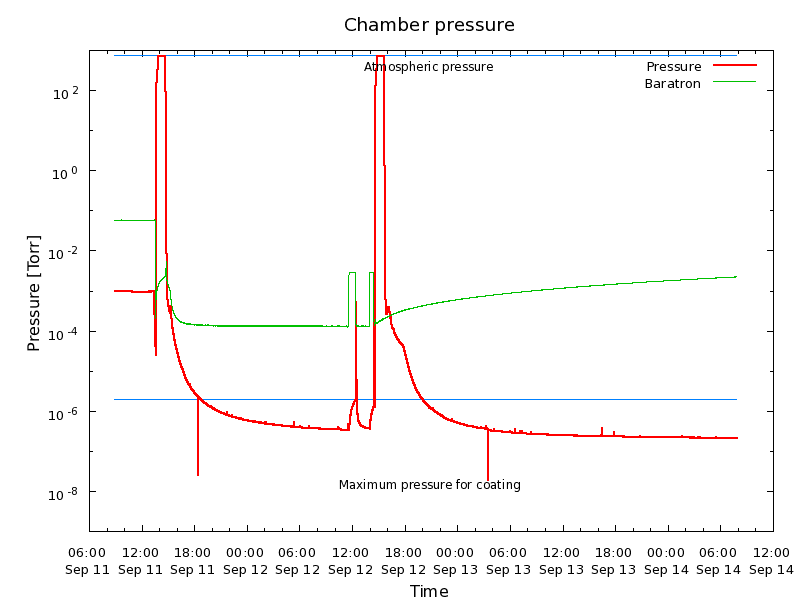
\includegraphics[width=0.8\linewidth]{figures/chamber/pressure.png}
  \caption{\footnotesize Plot representing the output from the continuous logging of chamber pressure. Red line is the pressure measured by a combined cold-cathode/penning gauge, that works well under both atmospheric pressure and low pressure. It will not function well during a coating. Green line is the MKS Baratron pressure gauge, that is precise in the $2\cdot10^{-4}$ -- $5\cdot10^{-2}$ Torr range.}
  \label{fig:chamber_pressure}
\end{figure}

The web server that continuously fetches the log file from the coating computer also gets information from the X-ray measurement computer in the basement. Information about measurement status and progress is posted to the same web site. This makes it possible to get the status about all the labs by a quick glance to the web site. The script running on the web server also has the option to send out a mail to pre-defined recipients if the pressure in the chamber is low enough to start a coating. This proved handy during the NuSTAR coatings, where coatings had to be started in the middle of the night. The web site and script running on the web server were produced during the NuSTAR coating campaign to make the production process easier.

The cathode shutters and ring are all controlled by the same motor controller, and is communicated to over the same serial cable. That is however opaque to the user. In order to open or close a specific shutter, the command \verb'osh #' or \verb'csh #' should be given for opening and closing shutter \verb'#', respectively. Alternatively, all shutters can be opened or closed using \verb'openallshutters' and \verb'closeallshutters'. The ring can be controlled using the commands \verb'mra speed angle' or \verb'mr speed steps', the first of which moves the ring at the speed given in steps/sec. at an angle given in degrees. The second does the same thing, except for changing the angle for steps. The motor controller has 668,000 steps in a complete rotation of the ring in the chamber and the speed of the ring should be between 0 and 15,000 steps/sec, otherwise the movement precision decreases. In a coating macro, the command \verb'mra speed angle' is used extensively as the main method to move the samples past the cathodes.% In chapter \ref{chap:multilab_details}, an extensive list of commands made for the control software can be found.

\subsection{Interfacing with cathode power supplies}
The power supplies used to run the cathodes in the multilab consist of two Advanced Energy Pinnacle 5/5 DC power supplies and one Advanced Energy Pinnacle Plus+ 5/5 pulsed-DC power supply. Each power supply has two channels, so can run two cathodes at same time. In order to communicate with power supplies, a special protocol running over serial has to be used. All other instruments in the multilab are communicated with by ControlServer and SPEC using basic text commands send over a serial connection.

The protocol is made for connecting all power supplies to the same serial connection, but in the multilab they are connected separately. The protocol requires each command to be packaged in a binary packet that includes power supply hardware address, length of packet, command, data and finally an XOR of the entire packet so the receiver can verify that the whole packet is there. The design of the packet can be seen in figure \ref{fig:ae_packet}. In the header, which is 8 bits long, the first 5 are the address of the power supply (set with a DIP switch on the back) and the remaining 3 bits describe the length of the packet. If the length in the header is set to 7 (111 in binary), the 'optional' byte is used to describe the actual length of the packet. The 'command' byte is a number between 0 and 255 (0 and FFh) in hexadecimal numbers. The 'checksum' byte is an XOR of the entire packet up until the 'chekcksum' byte. When the receiver gets a packet, it will do an XOR of the entire packet including the 'checksum' byte and if the result is 0, the packet is approved and processed.

This packet architecture is used to communicate back and forth between the ControlServer program and the power supplies. If a packet is approved, an ACK is send back in the form of the hex code 06h. The commands for the power supplies can either be to retrieve current status of some parameter, to set a parameter on the power supply, or to execute a command on the power supply. The entire communication protocol is transparent to the user and all user-level control of the power supplies can be achieved by user-level commands only.

\begin{figure}[!h]
  \center
  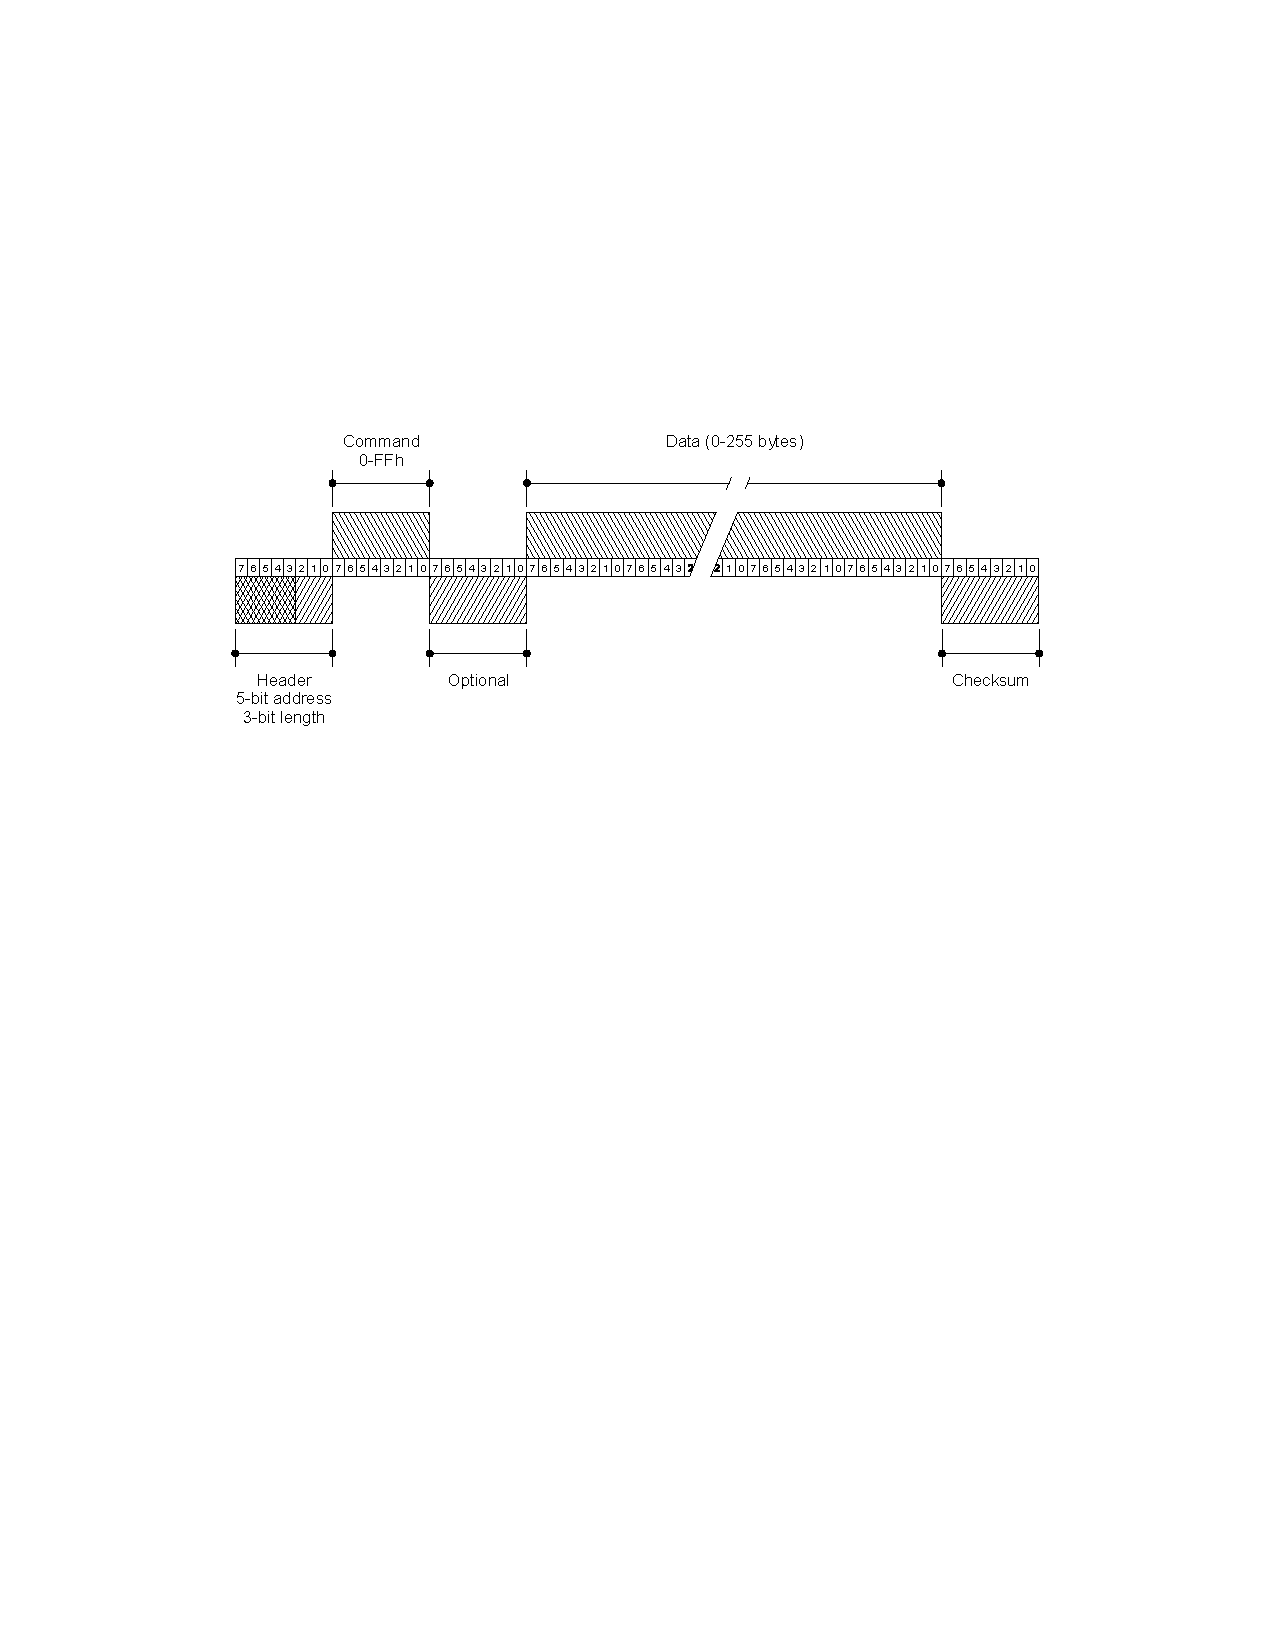
\includegraphics[width=0.9\linewidth]{figures/chamber/ae_packet.pdf}
\caption{\footnotesize Schematic of the principle of transmission data packets in the Advanced Energy communication protocol. Each number on the white line corresponds to one bit in the data packet, eight bits equals one byte. From \cite{Anonymous:zazNQqcS}}\label{fig:ae_packet}
\end{figure}

\subsection{Coating macro}
To produce a coating in the multilab chamber, a coating macro can be typed up and started in the main SPEC program as soon as the pressure is low enough ($\leq2\cdot10^{-6}$ Torr). An example of a simple coating macro, \verb'coat_singlelayer', can be seen here:

\begin{verbcode}
  def coat_singlelayer '
        if ($# != 1) {
                eprint "Start coating of singlelayer.\n"
                eprint "Usage: coat_singlelayer v(cath3)"
                exit
        }
        coating_start_log
        closevalve
        setflow 1 88
        openflow 1
        openmainflow
        print("Waiting for Ar flow to settle.\n")
        print("(60 seconds).\n")
        sleep(60)
        setpower 3 450
        print("Starting coating.\n")
        mra 90 10000
        sleep(2)
        pson 3
        sleep(5)
        osh 1
        print("Coating material 1, all plates.\n")
        mra -360 $1
        sleep(2)
        csh 1
        sleep(1)
        psoff 3
        mra -90 10000
        sleep(2)
        print("Coating over. Closing flow valve.\n")
        closemainflow
        closeflow 1
        openvalve
        coating_stop_log
        '
\end{verbcode}

Each step in the macro is described here:

\begin{description}
  \item[Error check] The macro starts out with an \verb|if| statement to make sure that there is one parameter after the user has called the macro.
  \item[coating\_start\_log] Sets the variable \verb|coating_starting=1| in the LogClient program and lets it know that it is time to start a log for a new coating.
  \item[closevalve] Closes valve to the cold cathode pressure gauge.
  \item[setflow 1 88] Sets flow output on flow controller 1 to 88 SCCM.
  \item[openflow 1] Opens flow controller 1.
  \item[openmainflow] Opens flow controllers to chamber.
  \item[Text output to user] Feedback should be given to user throughout the coating.
  \item[sleep(60)] Macro will wait for 60 seconds to let the pressure settle at $\sim$2.8 mTorr.
  \item[setpower 3 450] Power output is set to 450 W on power supply output 3, the first output on the second power supply.
  \item[mra 90 10000] Ring is moved 90\degr\ at a speed of 10,000 steps/sec. so the first sample is right before cathode 1.
  \item[pson 3] Power supply 3 is turned on.
  \item[osh 1] Shutter 1 to cathode 1 is opened.
  \item[mra -360 \$1] Ring is moved 360\degr\ at the speed given by the parameter which is set by the user when calling the macro.
  \item[csh 1] Shutter 1 is closed after ring is done moving.
  \item[psoff 3] Power supply 3 is turned off.
  \item[mra -90 10000] Ring is moved back to start position.
  \item[closemainflow] Main flow to flow controllers is turned off.
  \item[closeflow 1] Flow controller 1 flow is turned off.
  \item[openvalve] Valve to cold cathode pressure gauge is opened.
  \item[coating\_stop\_log] Sets the parameter \verb|coating_starting=0| in the LogClient program, which stops logging for that coating.
\end{description}

The macro will coat all samples in the ring with one layer of the material on cathode 1 at the speed given by the parameter after the macro call. Macros in SPEC are given in a C-type language and many types of loops and statements are implemented. The comprehensive manual for SPEC gives a good overview.

If the user wants to make more complicated multilayers, adjusting the macro example above into a graded-d type coating can of course seem daunting. For that reason, subfunctions are implemented that will coat e.g. 90\degr\ of the ring with cathode 3. The principle of the subfunction is as follows:

\begin{enumerate}
  \item From the start position of the ring where sample 1 is placed, the ring will move sample 1 between cathode 2 and 3.
  \item Turn on cathode 3 and open shutter.
  \item Move ring 90\degr\ given by input parameter.
  \item Close shutter 3 and turn off cathode.
  \item Move ring back to start position.
\end{enumerate}

The sample can then be coated by another cathode afterwards. If a larger batch requires coating at the same time, there are similar subfunctions for moving 180\degr\ and 360\degr.

The software also makes it possible to coat four different samples with four different coatings in the same coating run. By placing the samples at four different corners of the ring, each sample can have a coating applied separately. Flexible macros for that purpose are not yet implemented, but a template that can be changed into a specific purpose is the macro
\begin{verbcode}
  SPEC> coat_n_bilayers_4plates
\end{verbcode}
along with subfunction e.g.
\begin{verbcode}
  SPEC> abilayer_4_plates_c2c4($2,$3,$4,$5,$6,$7,$8,$9)
\end{verbcode}
that will coat four different constant-d coatings using cathode 2 and 4. It is possible to change any parameter for the power supplies or flow meters between each sample, so testing out a parameter space becomes significantly faster with this system.

For linearly graded-d coatings, an example is given below that shows the flexibility of the SPEC macro language.

\begin{verbcode}
  for (j=0;j<nlayers;j++){
    printf("\nStarting layer %g.\n",j+1)
    dlayer = dmin+(j)*(dmax-dmin)/(nlayers-1)
    dlayer1 = dlayer*gamma
    dlayer2 = dlayer*(1-gamma)
    speed1 = int(1/((dlayer1-sicorr)/sifact))
    speed2 = int(1/((dlayer2-wcorr)/wfact))
    coat_cath2_180 speed2
    coat_cath4_180 speed1
    }
\end{verbcode}

By defining \verb|nlayers| as the number of layers, \verb|dmin|, \verb|dmax| and \verb|gamma| of the coating along with calibration factors, the macro will for every layer calculate the speed for both materials and coat the correct thickness. Calibration factors are calculated as seen in section \ref{sec:coating_calib} where $a$ for W is \verb|wfact| and $b$ is \verb|wcorr|. The same principle can be used in other types of graded-d coatings, e.g. power-law gradings with $a$, $b$ and $c$ defined in $d_i = a/(b+i)^c$, where $d_i$ is the d-spacing of the i'th layer.
